\chapter{Medium voltage electrical system}

	\section{Beacon circuits}
	\paragraph{} In series circuit is selected for beacon circuits, illustrated in figure \ref{series}. This option is chosen because its advantages.
	\begin{figure}[H]
		\centering
		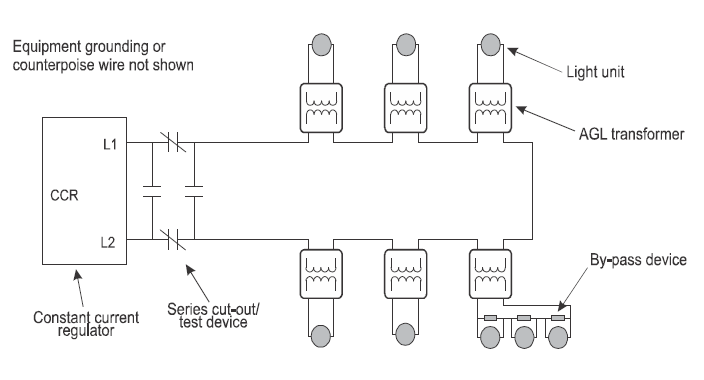
\includegraphics[clip, trim=0cm 0cm 0cm 0cm, width=0.7\textwidth]{./images/electric/series}
		\caption{Series lighting circuit.}
		\label{series}
	\end{figure}

	The constant current regulators of a series circuit, maintain a constant current independent of the load on the circuit. Thus, the same current will flow in a long circuit as in a shorter circuit and will remain the same even if some of the lamps fail. A short circuit across the output of a constant current regulator is a no-load condition and an open circuit is an overload. In a simple direct-connected series circuit, a lamp failure causes an open circuit; hence, it is necessary to provide an aerodrome ground lighting (AGL) transformer, as part of the circuit design, to maintain continuity of the circuit with lamp failure. Where a single transformer is used to supply several light units, as shown in Figure \ref{series}, a by-pass device is incorporated to ensure continuity on the secondary side.
	
	\subsection{Interleaving}
	\paragraph{} As a further means of assuring availability in case of failure, arrangement is made to enable switching to a spare regulator, as shown in Figure \ref{interleaved}. This method may be used where the regulator consists of the regulating component and input/output transformers. In the case of regulators that consist of only the regulating component, a rack mounted or plug-in design is used and availability is achieved by use of a spare regulator, Figure \ref{spare}, that can be readily installed in
	place of the failed regulator.
	
	\begin{figure}[H]
		\centering
		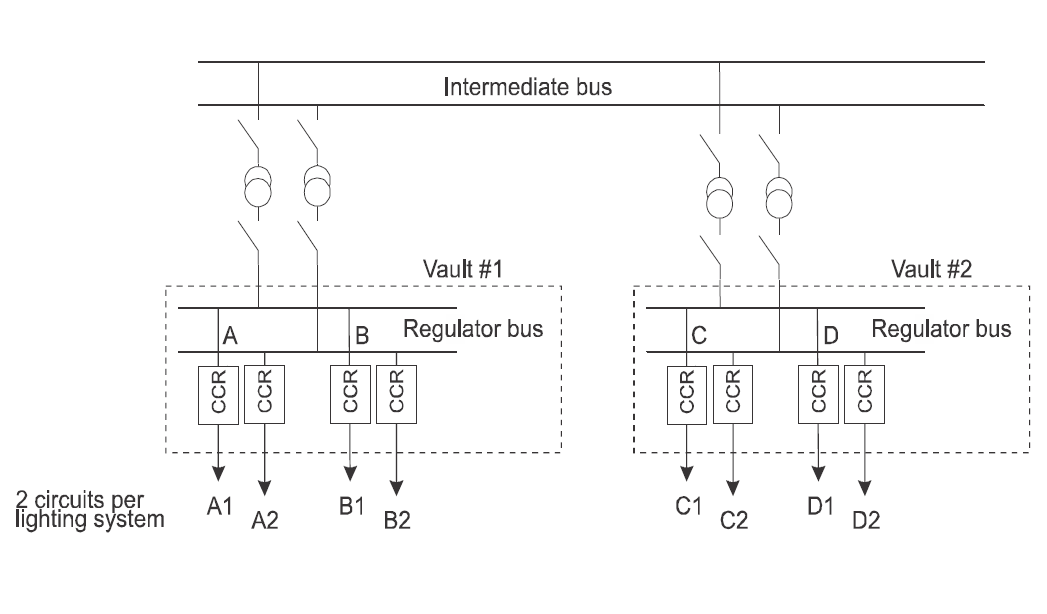
\includegraphics[clip, trim=0cm 0cm 0cm 0cm, width=0.8\textwidth]{./images/electric/interleaved}
		\caption{Provision of interleaved circuits.}
		\label{interleaved}
	\end{figure}

	\begin{figure}[H]
		\centering
		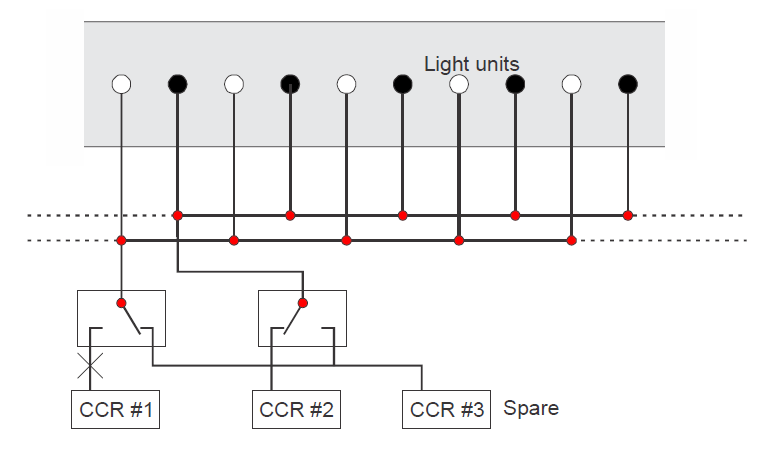
\includegraphics[clip, trim=0cm 0cm 0cm 0cm, width=0.7\textwidth]{./images/electric/spare}
		\caption{Use of a spare regulator.}
		\label{spare}
	\end{figure}
	
	
		\subsection{Runway centreline and touchdown lighting systems}
		\paragraph{} Annex 14, Volume I, requires that runway centreline lights show variable white to a distance of 900 m from the threshold, then alternating variable white and red from 900 m (or from the mid-point of the runway) to 300 m from the runway end after which only red is shown to the pilot. Figure \ref{rnwCentre} illustrates the interleaving for the first white only portion of the system. Similar interleaving would be used for the final all red portion.		
		
		\begin{figure}[H]
			\centering
			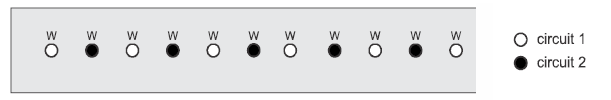
\includegraphics[clip, trim=0cm 0cm 0cm 0cm, width=0.7\textwidth]{./images/electric/rnwCentre}
			\caption{Runway centreline.}
			\label{rnwCentre}
		\end{figure}
		
		Interleaving to preserve spacing, Figure \ref{spacing}, is selected for the coded white/red portion of the system. This configuration, does not preserve the coding (with circuit failure the lights are either all red or all white), but does maintain an acceptable spacing for provision of a pattern of lights for centreline guidance (the spacing is doubled with circuit failure).
		
		\begin{figure}[H]
			\centering
			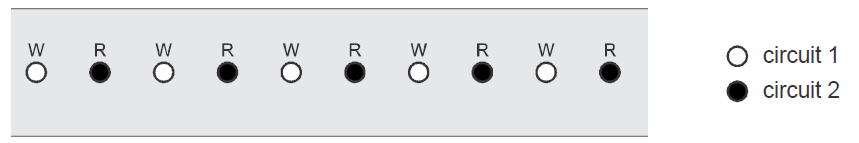
\includegraphics[clip, trim=0cm 0cm 0cm 0cm, width=0.7\textwidth]{./images/electric/spacing}
			\caption{Interleaving to preserve spacing.}
			\label{spacing}
		\end{figure}
	
		Figure \ref{touchdown} also illustrates the interleaving of runway touchdown zone lights. In this case three circuits will be used to preserve longitudinal spacing in case of one circuit failure.	
		\begin{figure}[H]
			\centering
			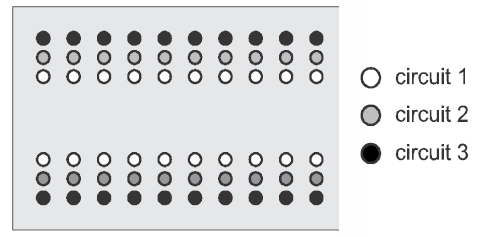
\includegraphics[clip, trim=0cm 0cm 0cm 0cm, width=0.7\textwidth]{./images/electric/touchdown}
			\caption{Interleaving by horizontal lines with three circuits.}
			\label{touchdown}
		\end{figure}
		
		
		\subsection{Taxiway centreline lighting system}
		\paragraph{} Taxiway centreline lighting circuits may be interleaved on those parts of the taxiway system that are considered as essential in category II/III conditions but, for economic reasons, a single circuit may be used for other taxiways.
		
		
		
		\subsection{Runway and taxiway centrelines lighting system}
		
		\subsection{Approach lighting system}
		
		\subsection{Touchdown zone lighting system}
		
		\subsection{Runway header lighting system}
		
		\subsection{RETIL electrical circuit}
		
		\subsection{PAPI electrical circuit}
		
		\subsection{Stop bar electrical circuit}
		
		\subsection{Signs electrical circuit}
		
	\section{Regulation chambers}
	
	\section{Wire channeling}
	
